\documentclass[twoside]{book}

% Packages required by doxygen
\usepackage{fixltx2e}
\usepackage{calc}
\usepackage{doxygen}
\usepackage[export]{adjustbox} % also loads graphicx
\usepackage{graphicx}
\usepackage[utf8]{inputenc}
\usepackage{makeidx}
\usepackage{multicol}
\usepackage{multirow}
\PassOptionsToPackage{warn}{textcomp}
\usepackage{textcomp}
\usepackage[nointegrals]{wasysym}
\usepackage[table]{xcolor}

% Font selection
\usepackage[T1]{fontenc}
\usepackage[scaled=.90]{helvet}
\usepackage{courier}
\usepackage{amssymb}
\usepackage{sectsty}
\renewcommand{\familydefault}{\sfdefault}
\allsectionsfont{%
  \fontseries{bc}\selectfont%
  \color{darkgray}%
}
\renewcommand{\DoxyLabelFont}{%
  \fontseries{bc}\selectfont%
  \color{darkgray}%
}
\newcommand{\+}{\discretionary{\mbox{\scriptsize$\hookleftarrow$}}{}{}}

% Page & text layout
\usepackage{geometry}
\geometry{%
  a4paper,%
  top=2.5cm,%
  bottom=2.5cm,%
  left=2.5cm,%
  right=2.5cm%
}
\tolerance=750
\hfuzz=15pt
\hbadness=750
\setlength{\emergencystretch}{15pt}
\setlength{\parindent}{0cm}
\setlength{\parskip}{3ex plus 2ex minus 2ex}
\makeatletter
\renewcommand{\paragraph}{%
  \@startsection{paragraph}{4}{0ex}{-1.0ex}{1.0ex}{%
    \normalfont\normalsize\bfseries\SS@parafont%
  }%
}
\renewcommand{\subparagraph}{%
  \@startsection{subparagraph}{5}{0ex}{-1.0ex}{1.0ex}{%
    \normalfont\normalsize\bfseries\SS@subparafont%
  }%
}
\makeatother

% Headers & footers
\usepackage{fancyhdr}
\pagestyle{fancyplain}
\fancyhead[LE]{\fancyplain{}{\bfseries\thepage}}
\fancyhead[CE]{\fancyplain{}{}}
\fancyhead[RE]{\fancyplain{}{\bfseries\leftmark}}
\fancyhead[LO]{\fancyplain{}{\bfseries\rightmark}}
\fancyhead[CO]{\fancyplain{}{}}
\fancyhead[RO]{\fancyplain{}{\bfseries\thepage}}
\fancyfoot[LE]{\fancyplain{}{}}
\fancyfoot[CE]{\fancyplain{}{}}
\fancyfoot[RE]{\fancyplain{}{\bfseries\scriptsize Generated by Doxygen }}
\fancyfoot[LO]{\fancyplain{}{\bfseries\scriptsize Generated by Doxygen }}
\fancyfoot[CO]{\fancyplain{}{}}
\fancyfoot[RO]{\fancyplain{}{}}
\renewcommand{\footrulewidth}{0.4pt}
\renewcommand{\chaptermark}[1]{%
  \markboth{#1}{}%
}
\renewcommand{\sectionmark}[1]{%
  \markright{\thesection\ #1}%
}

% Indices & bibliography
\usepackage{natbib}
\usepackage[titles]{tocloft}
\setcounter{tocdepth}{3}
\setcounter{secnumdepth}{5}
\makeindex

% Hyperlinks (required, but should be loaded last)
\usepackage{ifpdf}
\ifpdf
  \usepackage[pdftex,pagebackref=true]{hyperref}
\else
  \usepackage[ps2pdf,pagebackref=true]{hyperref}
\fi
\hypersetup{%
  colorlinks=true,%
  linkcolor=blue,%
  citecolor=blue,%
  unicode%
}

% Custom commands
\newcommand{\clearemptydoublepage}{%
  \newpage{\pagestyle{empty}\cleardoublepage}%
}

\usepackage{caption}
\captionsetup{labelsep=space,justification=centering,font={bf},singlelinecheck=off,skip=4pt,position=top}

%===== C O N T E N T S =====

\begin{document}

% Titlepage & ToC
\hypersetup{pageanchor=false,
             bookmarksnumbered=true,
             pdfencoding=unicode
            }
\pagenumbering{roman}
\begin{titlepage}
\vspace*{7cm}
\begin{center}%
{\Large 41012 }\\
\vspace*{1cm}
{\large Generated by Doxygen 1.8.11}\\
\end{center}
\end{titlepage}
\clearemptydoublepage
\tableofcontents
\clearemptydoublepage
\pagenumbering{arabic}
\hypersetup{pageanchor=true}

%--- Begin generated contents ---
\chapter{A Sample for 41012 Students}
\label{index}\hypertarget{index}{}Our main goal is the continuing progress in robotic research and the robotic industry. The main challenge we see at present is the software specific to robots, both its complexity and the sheer amount of it.\hypertarget{index_ac_doc_index_more_info}{}\section{Where to start}\label{index_ac_doc_index_more_info}

\begin{DoxyItemize}
\item This just divides the general instructions here for students
\end{DoxyItemize}\hypertarget{index_ac_doc_install}{}\section{Installation}\label{index_ac_doc_install}
\hypertarget{index_ac_doc_step1}{}\subsection{Step 1\+: Opening the box}\label{index_ac_doc_step1}
Openning the box\hypertarget{index_ac_doc_step2}{}\subsection{Step 2\+: Running applications}\label{index_ac_doc_step2}
The system needs three components running, please run\+:

\begin{DoxyVerb}./tests/controller_test ../cfg/sim.cfg
./tests/lo_up ../cfg/sim.cfg
./tests/acLoc ../cfg/sim.cfg\end{DoxyVerb}
 
\chapter{Hierarchical Index}
\section{Class Hierarchy}
This inheritance list is sorted roughly, but not completely, alphabetically\+:\begin{DoxyCompactList}
\item \contentsline{section}{Data\+Fusion}{\pageref{classDataFusion}}{}
\item \contentsline{section}{Ranger}{\pageref{classRanger}}{}
\begin{DoxyCompactList}
\item \contentsline{section}{Radar}{\pageref{classRadar}}{}
\item \contentsline{section}{Sonar}{\pageref{classSonar}}{}
\end{DoxyCompactList}
\end{DoxyCompactList}

\chapter{Class Index}
\section{Class List}
Here are the classes, structs, unions and interfaces with brief descriptions\+:\begin{DoxyCompactList}
\item\contentsline{section}{\hyperlink{classDataFusion}{Data\+Fusion} }{\pageref{classDataFusion}}{}
\item\contentsline{section}{\hyperlink{classRadar}{Radar} }{\pageref{classRadar}}{}
\item\contentsline{section}{\hyperlink{classRanger}{Ranger} }{\pageref{classRanger}}{}
\item\contentsline{section}{\hyperlink{classSonar}{Sonar} }{\pageref{classSonar}}{}
\end{DoxyCompactList}

\chapter{Class Documentation}
\hypertarget{classDataFusion}{}\section{Data\+Fusion Class Reference}
\label{classDataFusion}\index{Data\+Fusion@{Data\+Fusion}}
\subsection*{Public Member Functions}
\begin{DoxyCompactItemize}
\item 
void \hyperlink{classDataFusion_aa4afcc1feff6fdf9688d95ad640154cd}{start\+Fusion} (queue$<$ double $>$ \&stream1, queue$<$ double $>$ \&stream2, mutex \&mu, condition\+\_\+variable \&cond, int fuse\+Method)
\end{DoxyCompactItemize}
\subsection*{Protected Attributes}
\begin{DoxyCompactItemize}
\item 
double {\bfseries last\+Reading1\+\_\+}\hypertarget{classDataFusion_adf9b71d9520833a171900b7979210be1}{}\label{classDataFusion_adf9b71d9520833a171900b7979210be1}

\item 
double {\bfseries last\+Reading2\+\_\+}\hypertarget{classDataFusion_a3f4a0f8cdaaa4aa04bacb77aca0373d6}{}\label{classDataFusion_a3f4a0f8cdaaa4aa04bacb77aca0373d6}

\item 
double {\bfseries fused\+Data\+\_\+}\hypertarget{classDataFusion_a5dcf6bb23b44f3a5a953a4fdc5ec7579}{}\label{classDataFusion_a5dcf6bb23b44f3a5a953a4fdc5ec7579}

\item 
std\+::chrono\+::duration$<$ double $>$ {\bfseries last\+Fuse\+Time\+\_\+}\hypertarget{classDataFusion_a851740c7f918b3ec4195be061f8f275d}{}\label{classDataFusion_a851740c7f918b3ec4195be061f8f275d}

\item 
int {\bfseries fuse\+Rate\+\_\+}\hypertarget{classDataFusion_a4c036eccb8ed9b1a86ede0682e543704}{}\label{classDataFusion_a4c036eccb8ed9b1a86ede0682e543704}

\end{DoxyCompactItemize}


\subsection{Member Function Documentation}
\index{Data\+Fusion@{Data\+Fusion}!start\+Fusion@{start\+Fusion}}
\index{start\+Fusion@{start\+Fusion}!Data\+Fusion@{Data\+Fusion}}
\subsubsection[{\texorpdfstring{start\+Fusion(queue$<$ double $>$ \&stream1, queue$<$ double $>$ \&stream2, mutex \&mu, condition\+\_\+variable \&cond, int fuse\+Method)}{startFusion(queue< double > &stream1, queue< double > &stream2, mutex &mu, condition_variable &cond, int fuseMethod)}}]{\setlength{\rightskip}{0pt plus 5cm}void Data\+Fusion\+::start\+Fusion (
\begin{DoxyParamCaption}
\item[{queue$<$ double $>$ \&}]{stream1, }
\item[{queue$<$ double $>$ \&}]{stream2, }
\item[{mutex \&}]{mu, }
\item[{condition\+\_\+variable \&}]{cond, }
\item[{int}]{fuse\+Method}
\end{DoxyParamCaption}
)}\hypertarget{classDataFusion_aa4afcc1feff6fdf9688d95ad640154cd}{}\label{classDataFusion_aa4afcc1feff6fdf9688d95ad640154cd}
Start fusion member function. This accepts two references to queues (one for each sensor), mustex and condition variable and the selected fuse method Turn freqency (Hz) into a period

Lock mutex

When a new reading is entered into stream1, update the local variable

Copy variable

Pop from front of queue

Change varaible to notify that a new variable has been entered (3.\+c.\+ii produce a fused result on each new piece of sensor data)

When a new reading is entered into stream2, update the local variable

Copy variable

Pop from front of queue

Change varaible to notify that a new variable has been entered (3.\+c.\+ii produce a fused result on each new piece of sensor data)

Set current time to now

Calculate the duration since the last reading

True if enough time has passed or a new reading has been taken

Print out the reason why the event occured and reach sensor\textquotesingle{}s reading

If the selected fusion method is minimum, compare the two readings and assign the smallest to the fused\+Data\+\_\+ variable

Print the minimum to the console

If the selected fusion method is maximum, compare the two readings and assign the largest to the fused\+Data\+\_\+ variable

Print the maximum to the console

If the selected fusion method is average, add the two values and divide by two. Assign to fused\+Data\+\_\+ variable

Print the average to the console

Reset timer

Unlock Mutex. 

The documentation for this class was generated from the following files\+:\begin{DoxyCompactItemize}
\item 
data\+\_\+fusion.\+h\item 
data\+\_\+fusion.\+cpp\end{DoxyCompactItemize}

\hypertarget{classRadar}{}\section{Radar Class Reference}
\label{classRadar}\index{Radar@{Radar}}


{\ttfamily \#include $<$radar.\+h$>$}

Inheritance diagram for Radar\+:\begin{figure}[H]
\begin{center}
\leavevmode
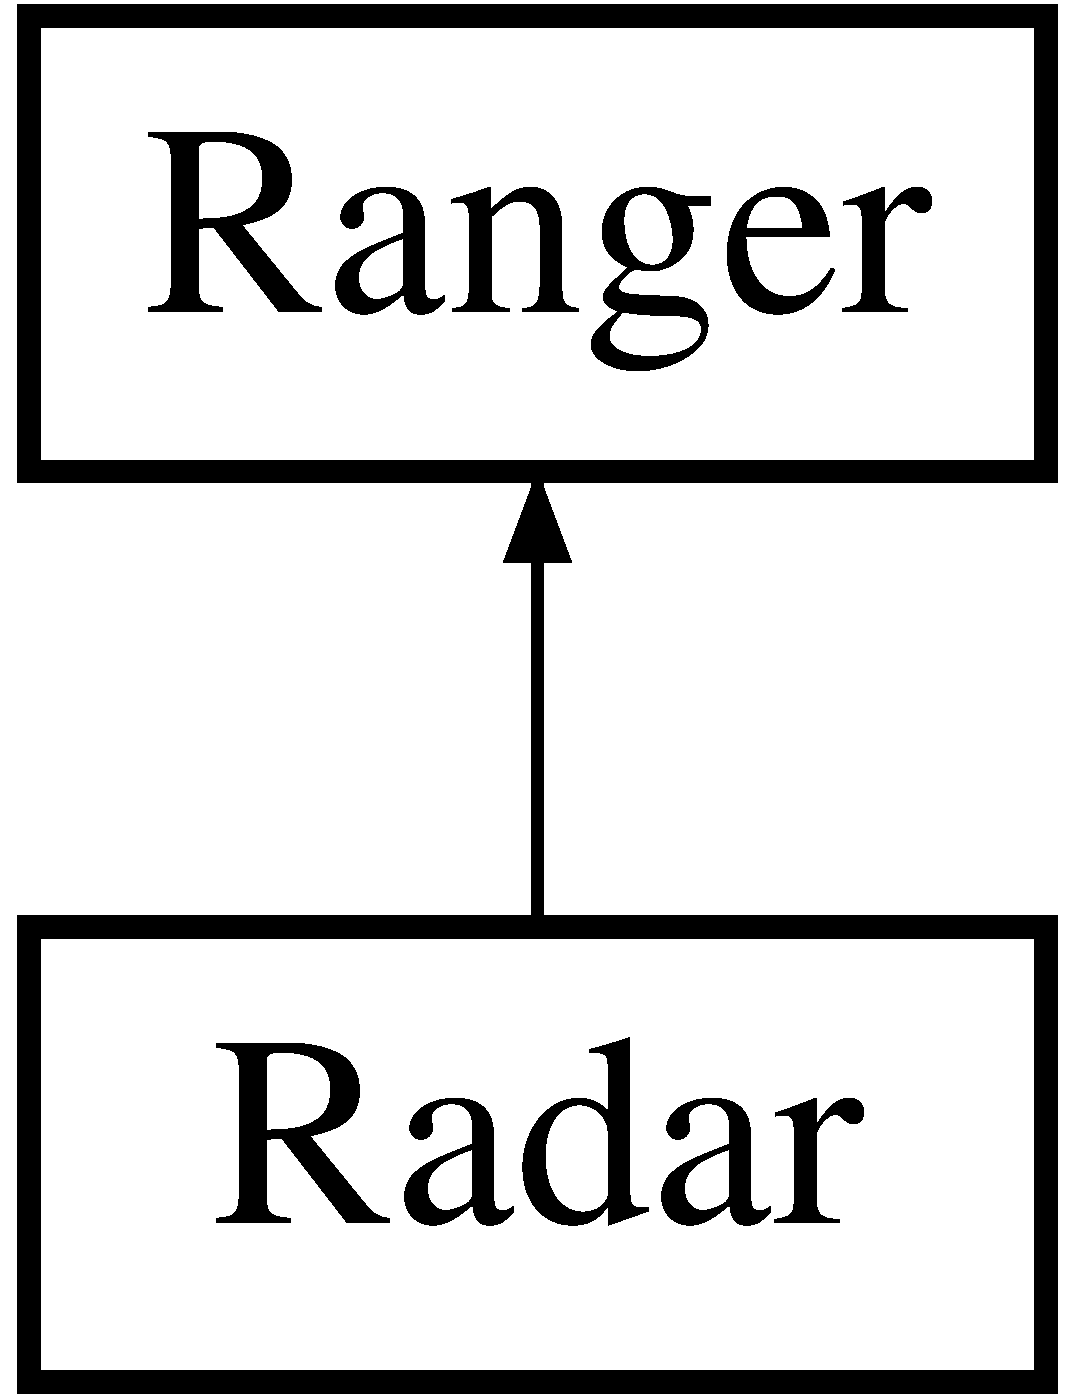
\includegraphics[height=2.000000cm]{classRadar}
\end{center}
\end{figure}
\subsection*{Public Member Functions}
\begin{DoxyCompactItemize}
\item 
\hyperlink{classRadar_aa1cfdbe0e024e68a14234069dbeb6808}{Radar} ()
\item 
bool {\bfseries set\+Fov} (double i)\hypertarget{classRadar_a3b1870e4bf92544b902785552a98a6e5}{}\label{classRadar_a3b1870e4bf92544b902785552a98a6e5}

\end{DoxyCompactItemize}
\subsection*{Additional Inherited Members}


\subsection{Detailed Description}
\hyperlink{radar_8h_source}{radar.\+h} Programming for Mechatronic systems Assignment 3

\begin{DoxyAuthor}{Author}
\+: Jamin Early 99133391 
\end{DoxyAuthor}
\begin{DoxyDate}{Date}
\+: Week 8 Autumn Semester 2018 
\end{DoxyDate}


\subsection{Constructor \& Destructor Documentation}
\index{Radar@{Radar}!Radar@{Radar}}
\index{Radar@{Radar}!Radar@{Radar}}
\subsubsection[{\texorpdfstring{Radar()}{Radar()}}]{\setlength{\rightskip}{0pt plus 5cm}Radar\+::\+Radar (
\begin{DoxyParamCaption}
{}
\end{DoxyParamCaption}
)}\hypertarget{classRadar_aa1cfdbe0e024e68a14234069dbeb6808}{}\label{classRadar_aa1cfdbe0e024e68a14234069dbeb6808}
When a radar object is initialised, it has all values set to default 

The documentation for this class was generated from the following files\+:\begin{DoxyCompactItemize}
\item 
radar.\+h\item 
radar.\+cpp\end{DoxyCompactItemize}

\hypertarget{classRanger}{}\section{Ranger Class Reference}
\label{classRanger}\index{Ranger@{Ranger}}
Inheritance diagram for Ranger\+:\begin{figure}[H]
\begin{center}
\leavevmode
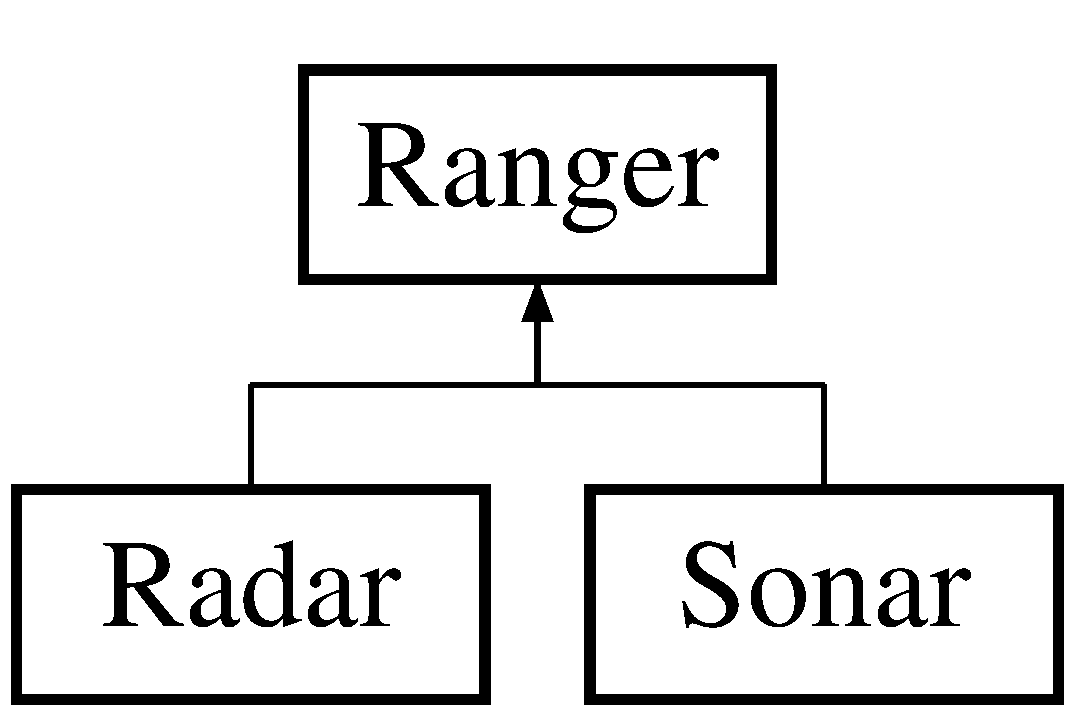
\includegraphics[height=2.000000cm]{classRanger}
\end{center}
\end{figure}
\subsection*{Public Member Functions}
\begin{DoxyCompactItemize}
\item 
\hyperlink{classRanger_a65e1b9530f370b95cd673690c5bf02b5}{Ranger} ()
\item 
bool \hyperlink{classRanger_a5cb6fe854af1751438b1a836c6703f3f}{set\+Baud\+Rate} (int i)
\item 
int \hyperlink{classRanger_abd9461cf6b81f879986e6ef79a1a7269}{get\+Baud\+Rate} ()
\item 
bool \hyperlink{classRanger_af9e1edce24012a056905fe4e41eca784}{set\+Tty\+A\+CM} (int i)
\item 
int \hyperlink{classRanger_a10d0c5f291b2cd850e6d82717d1e179d}{get\+Tty} ()
\item 
double \hyperlink{classRanger_a92538e7e7c3b5346501ed4116b6a96bb}{get\+Fov} ()
\item 
int {\bfseries get\+Data\+Rate} ()\hypertarget{classRanger_a76768ed2f954887a5d4aa48271fdee3d}{}\label{classRanger_a76768ed2f954887a5d4aa48271fdee3d}

\item 
double \hyperlink{classRanger_ab08a6310dee156f89fdd28256b1055e5}{get\+Min\+Distance} ()
\item 
double \hyperlink{classRanger_a8e5aaf0373980c5196b171fe3371190c}{get\+Max\+Distance} ()
\item 
void {\bfseries take\+Reading} (mutex \&mu, condition\+\_\+variable \&cond)\hypertarget{classRanger_af3c38e14a1cec55729563b5feebf1e6f}{}\label{classRanger_af3c38e14a1cec55729563b5feebf1e6f}

\end{DoxyCompactItemize}
\subsection*{Public Attributes}
\begin{DoxyCompactItemize}
\item 
queue$<$ double $>$ {\bfseries data\+Stream\+\_\+}\hypertarget{classRanger_a82f7e4ae6cd80d31baf5118a3df877ab}{}\label{classRanger_a82f7e4ae6cd80d31baf5118a3df877ab}

\end{DoxyCompactItemize}
\subsection*{Protected Member Functions}
\begin{DoxyCompactItemize}
\item 
bool \hyperlink{classRanger_ac191d948d1a1451927f0a856f131fed0}{set\+Max\+Distance} (double i)
\item 
bool \hyperlink{classRanger_ac3c89ae3ce2b6529f385ac356ca899f6}{set\+Min\+Distance} (double i)
\end{DoxyCompactItemize}
\subsection*{Protected Attributes}
\begin{DoxyCompactItemize}
\item 
std\+::chrono\+::duration$<$ double $>$ {\bfseries last\+Reading}\hypertarget{classRanger_a1bdab7210a1469ffff99eedd28f8b7e6}{}\label{classRanger_a1bdab7210a1469ffff99eedd28f8b7e6}

\item 
int {\bfseries baud\+Rate\+\_\+}\hypertarget{classRanger_aced6f17f9f3e14fb3a74d041d239d021}{}\label{classRanger_aced6f17f9f3e14fb3a74d041d239d021}

\item 
int {\bfseries tty\+A\+C\+M\+\_\+}\hypertarget{classRanger_affe5d5e2bcd736aa64fe36e8c305ebb6}{}\label{classRanger_affe5d5e2bcd736aa64fe36e8c305ebb6}

\item 
double {\bfseries fov\+\_\+}\hypertarget{classRanger_a43cc24e0ee22c92224eb6279f5da18d1}{}\label{classRanger_a43cc24e0ee22c92224eb6279f5da18d1}

\item 
double {\bfseries min\+Dist\+\_\+}\hypertarget{classRanger_a162f6de8033276f58138b46d39b78361}{}\label{classRanger_a162f6de8033276f58138b46d39b78361}

\item 
double {\bfseries max\+Dist\+\_\+}\hypertarget{classRanger_a46504fe73b39234252b9f93d9a6423a7}{}\label{classRanger_a46504fe73b39234252b9f93d9a6423a7}

\item 
int {\bfseries data\+Rate\+\_\+}\hypertarget{classRanger_a0e489954008a72da7eb57884b6ba5a73}{}\label{classRanger_a0e489954008a72da7eb57884b6ba5a73}

\end{DoxyCompactItemize}


\subsection{Constructor \& Destructor Documentation}
\index{Ranger@{Ranger}!Ranger@{Ranger}}
\index{Ranger@{Ranger}!Ranger@{Ranger}}
\subsubsection[{\texorpdfstring{Ranger()}{Ranger()}}]{\setlength{\rightskip}{0pt plus 5cm}Ranger\+::\+Ranger (
\begin{DoxyParamCaption}
{}
\end{DoxyParamCaption}
)}\hypertarget{classRanger_a65e1b9530f370b95cd673690c5bf02b5}{}\label{classRanger_a65e1b9530f370b95cd673690c5bf02b5}
ranger.\+cpp Programming for Mechatronic systems Assignment 3

\begin{DoxyAuthor}{Author}
\+: Jamin Early 99133391 
\end{DoxyAuthor}
\begin{DoxyDate}{Date}
\+: Week 8 Autumn Semester 2018 
\end{DoxyDate}


\subsection{Member Function Documentation}
\index{Ranger@{Ranger}!get\+Baud\+Rate@{get\+Baud\+Rate}}
\index{get\+Baud\+Rate@{get\+Baud\+Rate}!Ranger@{Ranger}}
\subsubsection[{\texorpdfstring{get\+Baud\+Rate()}{getBaudRate()}}]{\setlength{\rightskip}{0pt plus 5cm}int Ranger\+::get\+Baud\+Rate (
\begin{DoxyParamCaption}
{}
\end{DoxyParamCaption}
)}\hypertarget{classRanger_abd9461cf6b81f879986e6ef79a1a7269}{}\label{classRanger_abd9461cf6b81f879986e6ef79a1a7269}
Returns baud rate \index{Ranger@{Ranger}!get\+Fov@{get\+Fov}}
\index{get\+Fov@{get\+Fov}!Ranger@{Ranger}}
\subsubsection[{\texorpdfstring{get\+Fov()}{getFov()}}]{\setlength{\rightskip}{0pt plus 5cm}double Ranger\+::get\+Fov (
\begin{DoxyParamCaption}
{}
\end{DoxyParamCaption}
)}\hypertarget{classRanger_a92538e7e7c3b5346501ed4116b6a96bb}{}\label{classRanger_a92538e7e7c3b5346501ed4116b6a96bb}
Returns field of view \index{Ranger@{Ranger}!get\+Max\+Distance@{get\+Max\+Distance}}
\index{get\+Max\+Distance@{get\+Max\+Distance}!Ranger@{Ranger}}
\subsubsection[{\texorpdfstring{get\+Max\+Distance()}{getMaxDistance()}}]{\setlength{\rightskip}{0pt plus 5cm}double Ranger\+::get\+Max\+Distance (
\begin{DoxyParamCaption}
{}
\end{DoxyParamCaption}
)}\hypertarget{classRanger_a8e5aaf0373980c5196b171fe3371190c}{}\label{classRanger_a8e5aaf0373980c5196b171fe3371190c}
Returns maximum distance \index{Ranger@{Ranger}!get\+Min\+Distance@{get\+Min\+Distance}}
\index{get\+Min\+Distance@{get\+Min\+Distance}!Ranger@{Ranger}}
\subsubsection[{\texorpdfstring{get\+Min\+Distance()}{getMinDistance()}}]{\setlength{\rightskip}{0pt plus 5cm}double Ranger\+::get\+Min\+Distance (
\begin{DoxyParamCaption}
{}
\end{DoxyParamCaption}
)}\hypertarget{classRanger_ab08a6310dee156f89fdd28256b1055e5}{}\label{classRanger_ab08a6310dee156f89fdd28256b1055e5}
Returns minimum distance \index{Ranger@{Ranger}!get\+Tty@{get\+Tty}}
\index{get\+Tty@{get\+Tty}!Ranger@{Ranger}}
\subsubsection[{\texorpdfstring{get\+Tty()}{getTty()}}]{\setlength{\rightskip}{0pt plus 5cm}int Ranger\+::get\+Tty (
\begin{DoxyParamCaption}
{}
\end{DoxyParamCaption}
)}\hypertarget{classRanger_a10d0c5f291b2cd850e6d82717d1e179d}{}\label{classRanger_a10d0c5f291b2cd850e6d82717d1e179d}
Returns port \index{Ranger@{Ranger}!set\+Baud\+Rate@{set\+Baud\+Rate}}
\index{set\+Baud\+Rate@{set\+Baud\+Rate}!Ranger@{Ranger}}
\subsubsection[{\texorpdfstring{set\+Baud\+Rate(int i)}{setBaudRate(int i)}}]{\setlength{\rightskip}{0pt plus 5cm}bool Ranger\+::set\+Baud\+Rate (
\begin{DoxyParamCaption}
\item[{int}]{i}
\end{DoxyParamCaption}
)}\hypertarget{classRanger_a5cb6fe854af1751438b1a836c6703f3f}{}\label{classRanger_a5cb6fe854af1751438b1a836c6703f3f}
Sets baud rate. Returns if sane \index{Ranger@{Ranger}!set\+Max\+Distance@{set\+Max\+Distance}}
\index{set\+Max\+Distance@{set\+Max\+Distance}!Ranger@{Ranger}}
\subsubsection[{\texorpdfstring{set\+Max\+Distance(double i)}{setMaxDistance(double i)}}]{\setlength{\rightskip}{0pt plus 5cm}bool Ranger\+::set\+Max\+Distance (
\begin{DoxyParamCaption}
\item[{double}]{i}
\end{DoxyParamCaption}
)\hspace{0.3cm}{\ttfamily [protected]}}\hypertarget{classRanger_ac191d948d1a1451927f0a856f131fed0}{}\label{classRanger_ac191d948d1a1451927f0a856f131fed0}
Sets maximum distance. Returns if sane \index{Ranger@{Ranger}!set\+Min\+Distance@{set\+Min\+Distance}}
\index{set\+Min\+Distance@{set\+Min\+Distance}!Ranger@{Ranger}}
\subsubsection[{\texorpdfstring{set\+Min\+Distance(double i)}{setMinDistance(double i)}}]{\setlength{\rightskip}{0pt plus 5cm}bool Ranger\+::set\+Min\+Distance (
\begin{DoxyParamCaption}
\item[{double}]{i}
\end{DoxyParamCaption}
)\hspace{0.3cm}{\ttfamily [protected]}}\hypertarget{classRanger_ac3c89ae3ce2b6529f385ac356ca899f6}{}\label{classRanger_ac3c89ae3ce2b6529f385ac356ca899f6}
Sets minimum distance. Returns if sane \index{Ranger@{Ranger}!set\+Tty\+A\+CM@{set\+Tty\+A\+CM}}
\index{set\+Tty\+A\+CM@{set\+Tty\+A\+CM}!Ranger@{Ranger}}
\subsubsection[{\texorpdfstring{set\+Tty\+A\+C\+M(int i)}{setTtyACM(int i)}}]{\setlength{\rightskip}{0pt plus 5cm}bool Ranger\+::set\+Tty\+A\+CM (
\begin{DoxyParamCaption}
\item[{int}]{i}
\end{DoxyParamCaption}
)}\hypertarget{classRanger_af9e1edce24012a056905fe4e41eca784}{}\label{classRanger_af9e1edce24012a056905fe4e41eca784}
Sets port. Returns if sane 

The documentation for this class was generated from the following files\+:\begin{DoxyCompactItemize}
\item 
ranger.\+h\item 
ranger.\+cpp\end{DoxyCompactItemize}

\hypertarget{classSonar}{}\section{Sonar Class Reference}
\label{classSonar}\index{Sonar@{Sonar}}


{\ttfamily \#include $<$sonar.\+h$>$}

Inheritance diagram for Sonar\+:\begin{figure}[H]
\begin{center}
\leavevmode
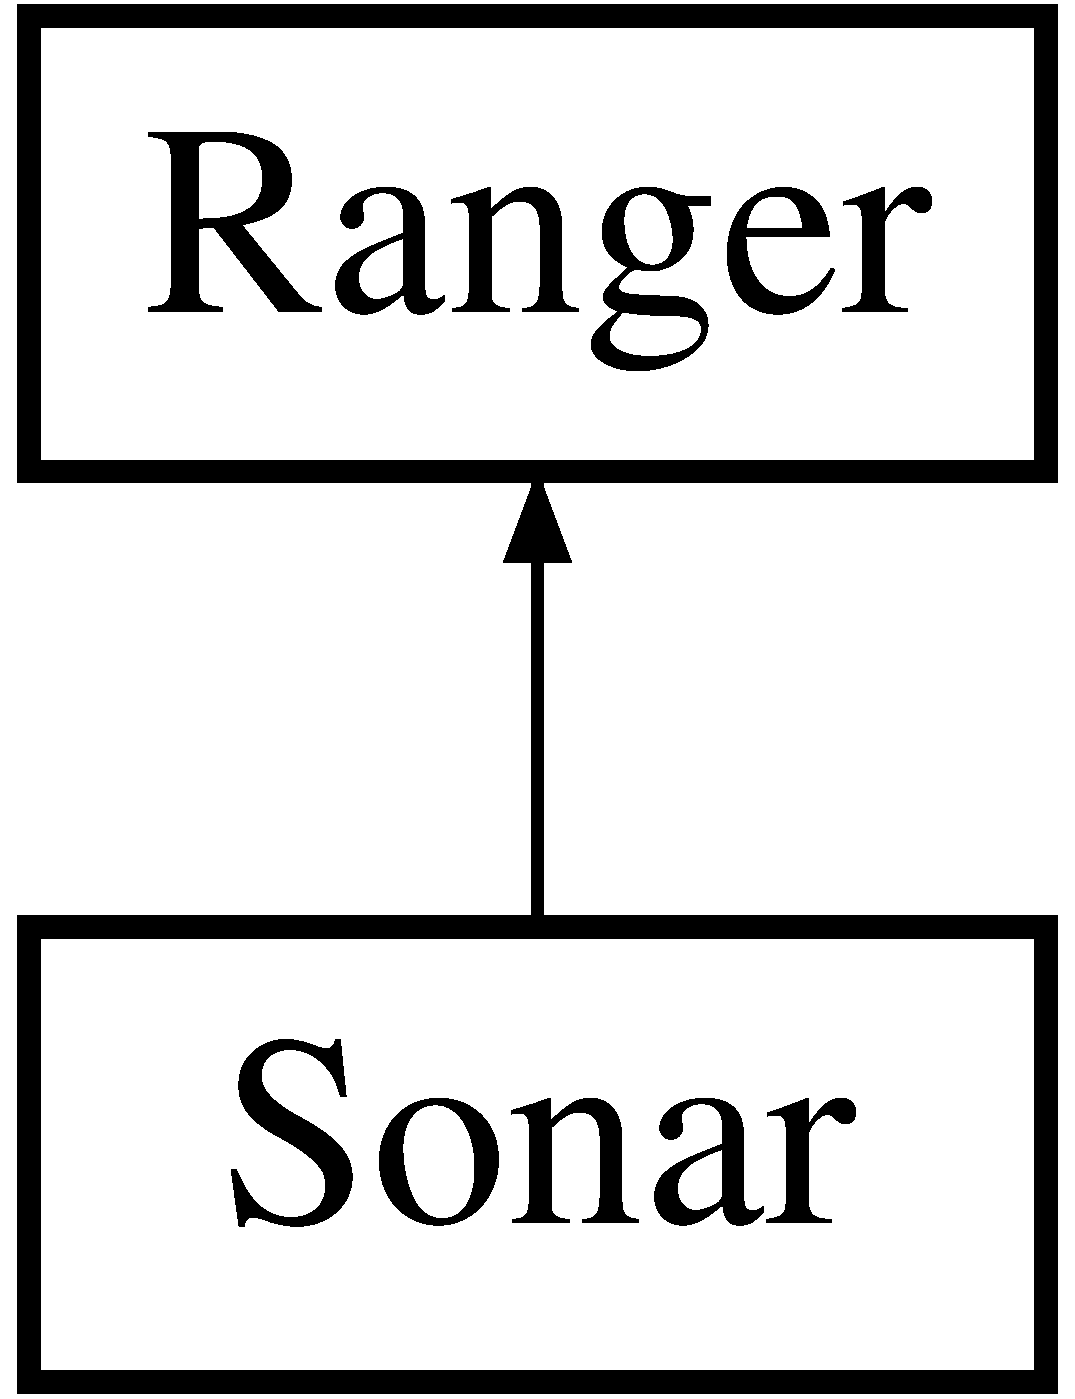
\includegraphics[height=2.000000cm]{classSonar}
\end{center}
\end{figure}
\subsection*{Additional Inherited Members}


\subsection{Detailed Description}
\hyperlink{sonar_8h_source}{sonar.\+h} Programming for Mechatronic systems Assignment 3

\begin{DoxyAuthor}{Author}
\+: Jamin Early 99133391 
\end{DoxyAuthor}
\begin{DoxyDate}{Date}
\+: Week 8 Autumn Semester 2018 
\end{DoxyDate}


The documentation for this class was generated from the following files\+:\begin{DoxyCompactItemize}
\item 
sonar.\+h\item 
sonar.\+cpp\end{DoxyCompactItemize}

%--- End generated contents ---

% Index
\backmatter
\newpage
\phantomsection
\clearemptydoublepage
\addcontentsline{toc}{chapter}{Index}
\printindex

\end{document}
